% !TEX root = ../main.tex
\chapter{DIS Platform Context and Architecture}
\label{chap:chapter2}
\section*{Introduction}
This chapter presents the background required to understand the solutions
developed during the internship. It first positions Data Intelligence Services
(DIS) within Oracle and explains the platform's purpose. It then introduces the
partner and tenant operating model, the principal functional layers, and the
cloud-native software architecture. Development technologies and engineering
tools are presented separately in Chapter~\ref{chap:chapter3}, where they are
directly related to the implemented solution.

\section{Data Intelligence Services Foundations}

\subsection{Position within Oracle}
Chapter~\ref{chap:general-project-context} introduced Oracle and the DIS team
from an organizational perspective. At platform level, the relevant
relationship is between Oracle's infrastructure organization and its Global
Business Units:
\begin{itemize}
    \item the greater Oracle organization, which focuses primarily on infrastructure and platform services such as OCI.
    \item Global Business Units (GBUs), which deliver SaaS solutions tailored to specific industry domains such as healthcare, finance, hospitality, and retail.
\end{itemize}
\begin{figure}[H]
    \centering
    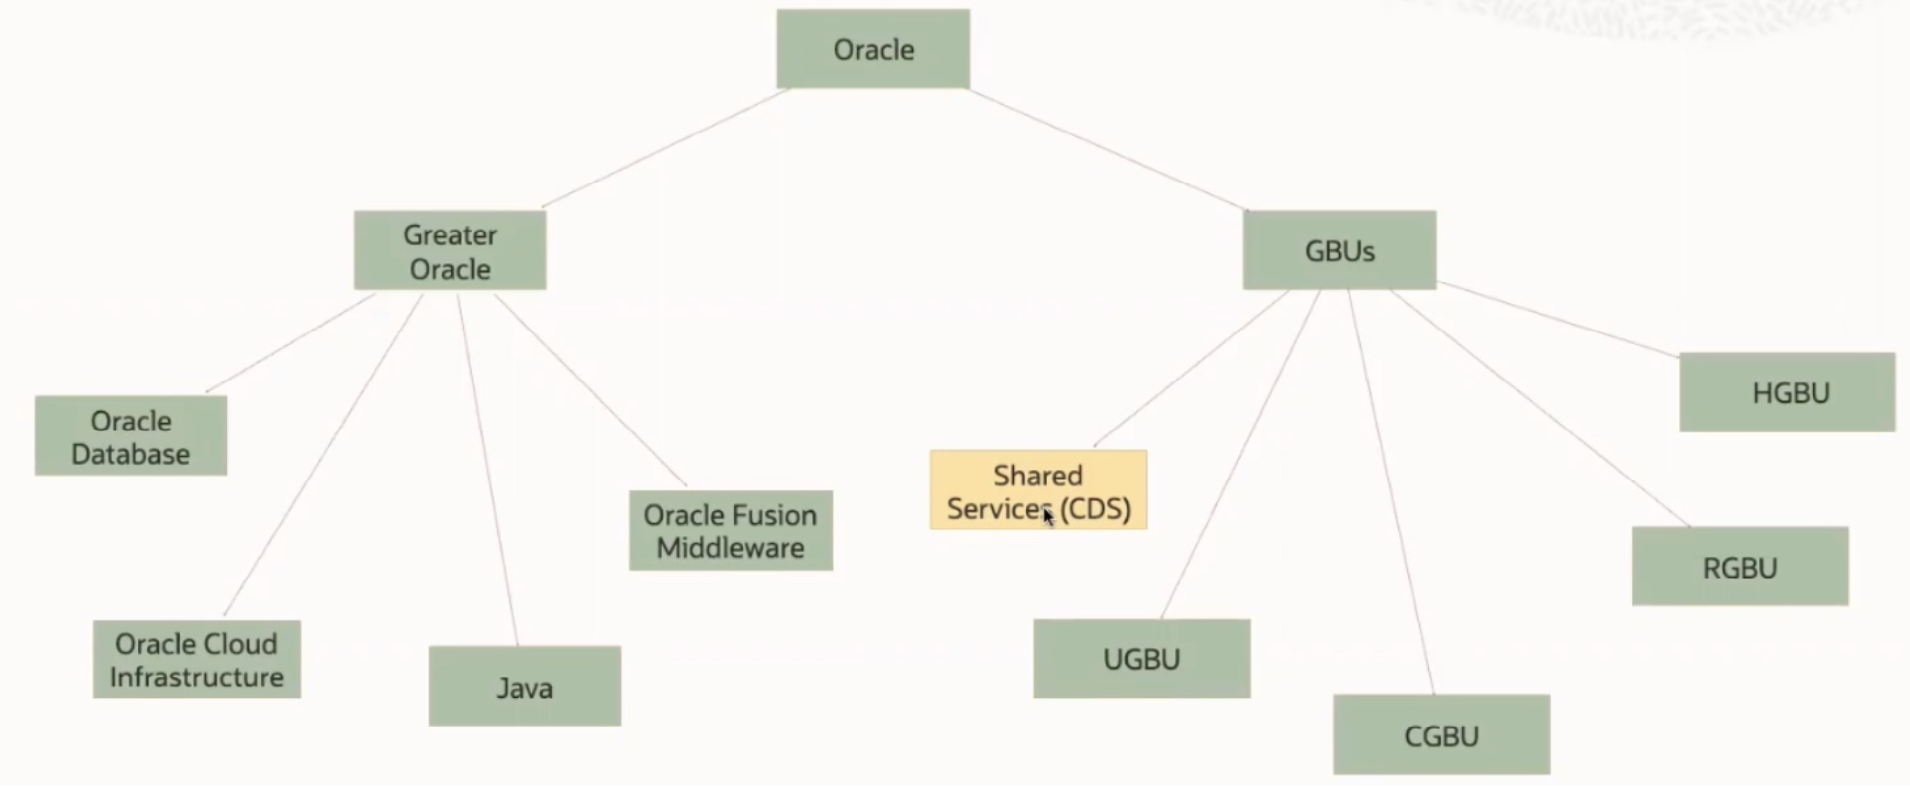
\includegraphics[width=0.8\textwidth]{Figures/oracle entities.png}
    \caption{Oracle entities}
    \label{fig:oracle-entities}
\end{figure}

Shared Services connects these two domains by providing common capabilities to
GBU product teams. Within this structure, DIS acts as the managed analytics
platform between industry-specific SaaS applications and the OCI services on
which their data workloads depend. Figure~\ref{fig:oracle-entities} summarizes
this positioning.

\subsection{Regional Availability}
DIS is intended to be deployed in the OCI regions where the required supporting services are available. Deployment priorities are determined according to forecast demand from GBU partners and their regional requirements. Figure~\ref{fig:dis-region-availability} presents the planned availability of DIS across the relevant regions.
\begin{figure}[H]
    \centering
    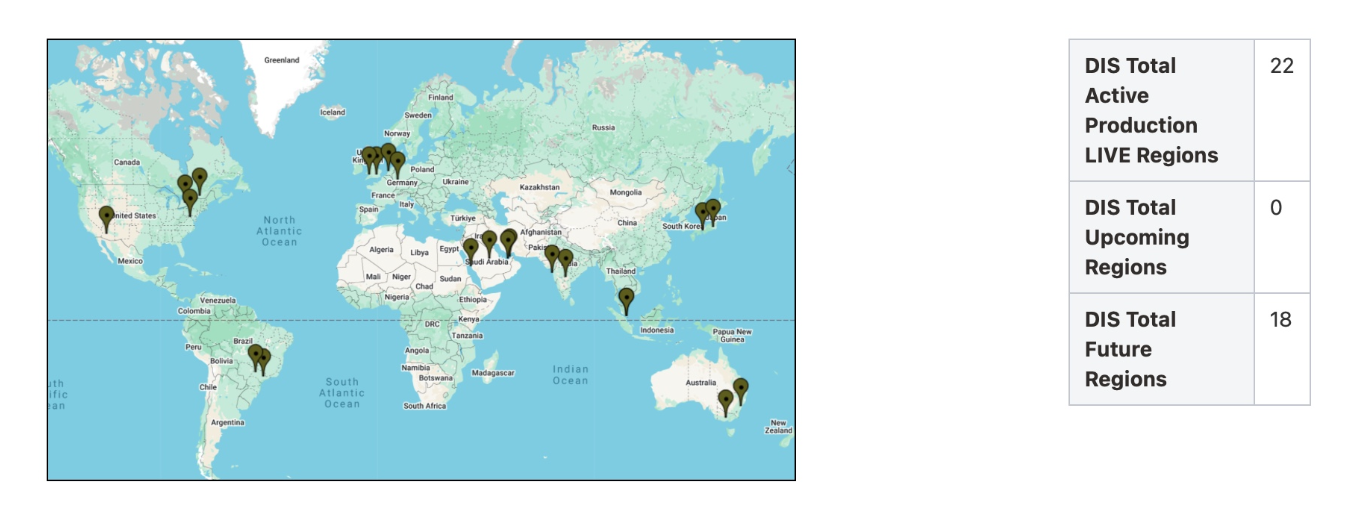
\includegraphics[width=0.8\textwidth]{Figures/DIS Region Availability.png}
    \caption{DIS Region Availability}
    \label{fig:dis-region-availability}
\end{figure}

\subsection{Data Intelligence Concepts}
Data intelligence refers to an organization's ability to collect, process, analyze, and interpret data in order to generate actionable insights. It combines tools, technologies, governance practices, and analytical methods that transform raw data into information that supports decision-making. By using their data assets effectively, organizations can improve operational efficiency, identify opportunities, and support strategic initiatives. In a data-driven environment, these capabilities are important for sustaining innovation and delivering value across business units.

\subsection{Purpose and Role}
DIS is an internal Oracle platform that provides product teams with a reusable analytics stack. Instead of requiring each GBU to build its analytics infrastructure from the ground up, DIS provides shared capabilities for data ingestion, storage, processing, machine learning, and visualization. A partner SaaS application can therefore integrate dashboards, reports, predictive models, and analytics pages through DIS rather than developing and operating each capability independently.

From a business perspective, Oracle's GBUs deliver SaaS solutions to their customers, while DIS provides the analytics layer embedded within those offerings. The platform provisions and manages services such as Oracle Analytics Server (OAS), Autonomous Data Warehouse (ADW), and Apache Spark, together with other analytics and data-processing components. End users access these capabilities through the corresponding SaaS applications.

By leveraging DIS for analytics-intensive workloads, partners benefit from the following advantages:

\begin{itemize}
    \item Avoid building and maintaining a custom analytics technology stack.
    \item Gain access to a cost-effective and scalable architecture tailored to analytics requirements.
    \item Focus on developing advanced machine learning capabilities using built-in frameworks and libraries.
    \item Maintain full control and flexibility over data ingestion, storage, processing, and visualization.
    \item Reduce Cloud Service Security Approval Process (CSSAP) overhead by adopting DIS's pre-approved architectural patterns.
\end{itemize}

\section{Platform Operating Model}

\subsection{Multi-Tenancy and Resource Isolation}

Multi-tenancy allows DIS to serve several partners and customer
environments while sharing common platform services. In this context, a
\textbf{tenant} represents an isolated logical environment with its own
identifier, configuration, enabled services, identities, analytics
resources, connections, and operational status. A \textbf{partner}
represents the GBU or SaaS application that uses DIS and may manage several
tenants.

An OCI tenancy is different from a DIS tenant. The OCI tenancy is the
cloud-account and root-resource boundary containing infrastructure such as
compartments, networks, Kubernetes clusters, databases, and Object Storage.
A DIS tenant is created at the application-platform level and represents
one logically isolated customer or application environment. Figure~\ref{fig:oci-tenancy-dis-tenant}
illustrates these different levels.

\begin{figure}[H]
    \centering
    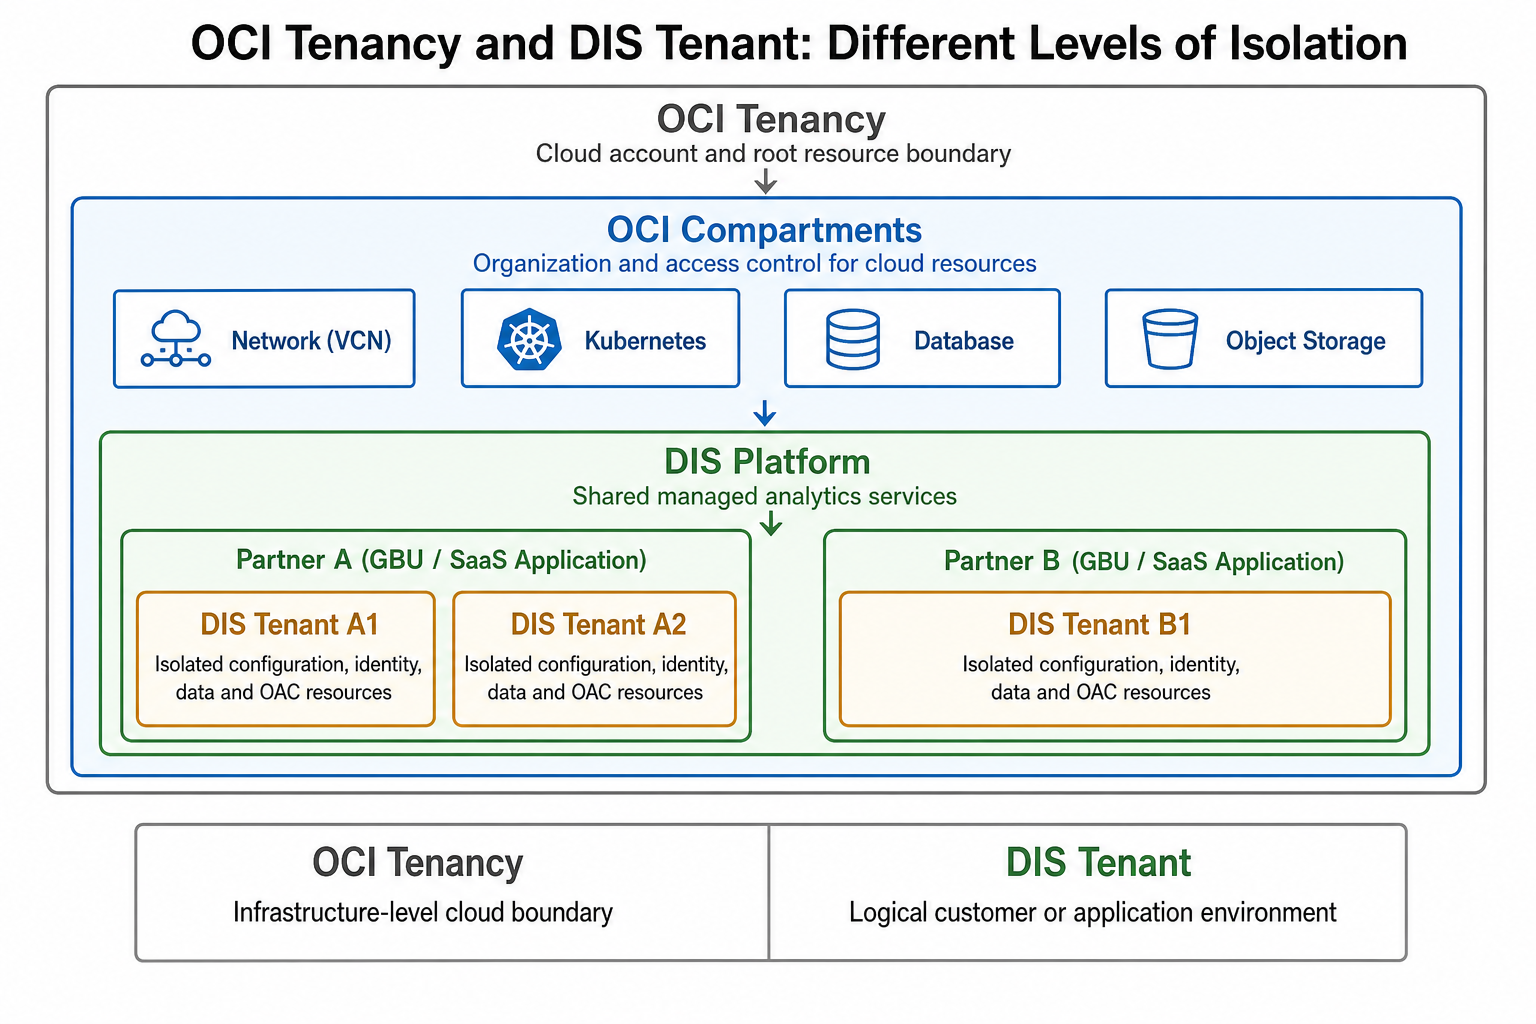
\includegraphics[width=\textwidth]
    {Figures/oci_tenancy_vs_dis_tenant.png}
    \caption{Difference between an OCI tenancy and a DIS tenant}
    \label{fig:oci-tenancy-dis-tenant}
\end{figure}

During onboarding, DIS provisions only the components declared in each
tenant's deployment template, such as a data lake, OAS, or OAC. Isolation
is enforced through tenant-specific identities and permissions, controlled
resource organization, network rules, and separate data and configuration
contexts. Consequently, operations performed for one tenant should not
affect the resources or data of another tenant.

\subsection{Partner and Tenant Provisioning Lifecycle}

Before a tenant can consume analytics services, DIS follows a controlled
provisioning lifecycle. This lifecycle separates the configuration shared
by a partner from the resources dedicated to each tenant:

\begin{enumerate}
    \item \textbf{Partner registration:} the partner is declared in DIS
    together with its authorized products, deployment templates, service
    limits, and infrastructure configuration.

    \item \textbf{Partner onboarding:} versioned application artifacts and
    container images are validated and stored so that they can later be
    deployed consistently for the partner's tenants.

    \item \textbf{Tenant registration:} a tenant identifier is created and
    associated with the corresponding partner. This identifier isolates the
    tenant's configuration and tracks subsequent lifecycle operations.

    \item \textbf{Tenant onboarding:} the partner submits an onboarding
    request that specifies the required products and deployment templates.
    The Orchestration Service validates the request and coordinates the
    services that provision and configure the requested resources.
\end{enumerate}

\subsubsection{Partner Artifact Packaging}

Before tenant provisioning, the partner prepares product-specific
configuration and analytics resources, such as semantic models,
visualization content, metadata, and deployment configuration. These
resources are packaged into a versioned container image based on a
platform-approved base image.

A continuous integration pipeline builds and publishes the image to an
authorized container registry. The DIS partner-artifact onboarding pipeline
then retrieves the image, validates its structure and metadata, and stores
its contents in the platform's artifact repository. The validated artifacts
can subsequently be used during tenant onboarding and upgrade operations.
This mechanism provides consistent packaging, traceable versioning, and
repeatable deployment across tenant environments.

Figure~\ref{fig:tenant-onboarding-workflow} summarizes the tenant onboarding
workflow, from submission of the request to the creation and configuration
of the tenant environment.

\begin{figure}[H]
    \centering
    \IfFileExists{Figures/tenant_onboarding_workflow.png}{%
        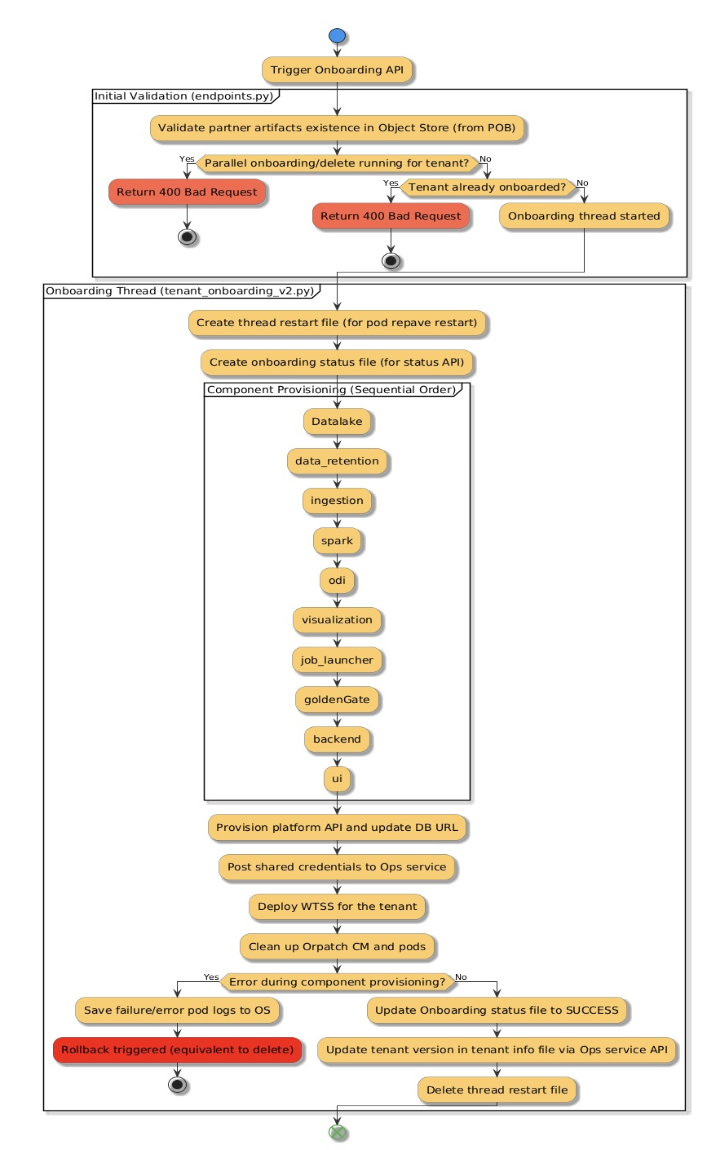
\includegraphics[width=0.6\textwidth]
        {Figures/tenant_onboarding_workflow.png}%
    }{%
        \fbox{\parbox[c][5cm][c]{0.88\textwidth}{\centering
        Insert the sanitized Tenant Onboarding Workflow figure here.}}%
    }
    \caption{Tenant Onboarding Workflow}
    \label{fig:tenant-onboarding-workflow}
\end{figure}

\section{Functional Architecture}

From a functional perspective, DIS organizes the analytics lifecycle into
three complementary layers: data ingestion, data storage and processing, and
visualization. Their relationship is shown in
Figure~\ref{fig:gbu_architecture}.

\begin{figure}[H]
    \centering
    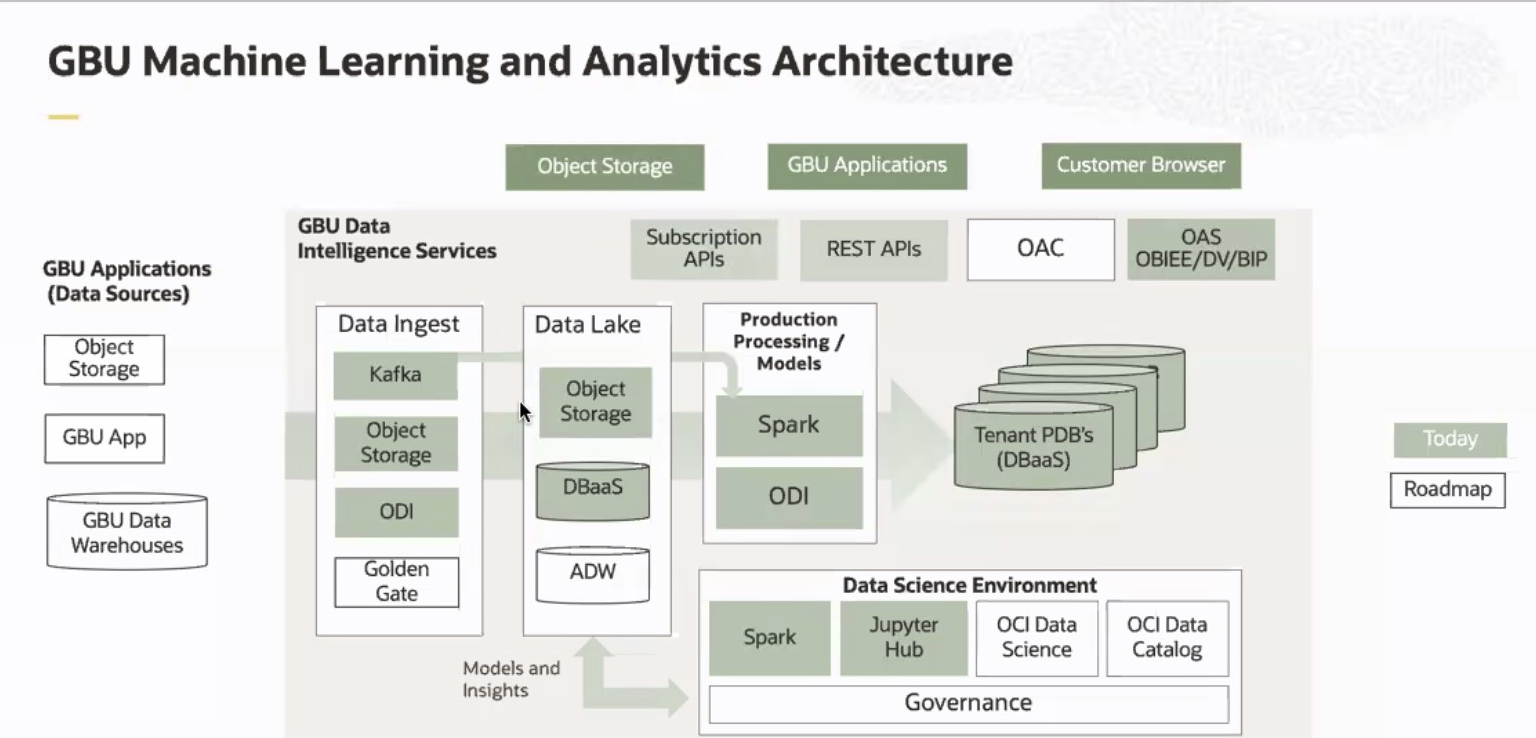
\includegraphics[width=0.9\textwidth]{Figures/gbu_architecture.png}
    \caption{GBU Analytics and Machine Learning Architecture}
    \label{fig:gbu_architecture}
\end{figure}

\subsection{Data Ingestion}

The data ingestion layer supports multiple methods for collecting data from Oracle SaaS applications and partner systems:

\begin{itemize}
    \item \textbf{REST Ingestion:} Data can be streamed into the platform using REST endpoints. These endpoints perform inline validation and Personally Identifiable Information (PII) detection during ingestion.

    \item \textbf{Oracle Data Integrator (ODI):} ODI is used to extract and load data from partner Database-as-a-Service (DBaaS) systems. It supports standard Extract, Transform, and Load (ETL) operations.

    \item \textbf{Direct Upload to Object Storage:} Large datasets, such as log files and historical data, can be uploaded directly to Oracle Object Storage for later processing.
\end{itemize}

\subsection{Data Storage and Processing}

The data processing layer provides distributed data processing using Apache Spark. It executes machine learning pipelines and data transformation jobs, storing the processed results in Oracle DBaaS. Spark jobs are tenant-isolated and are designed to periodically retrain machine learning models using historical data stored in Object Storage.

\subsection{Visualization and Data Analysis}

After data has been processed and stored, Oracle Business Intelligence Enterprise Edition (OBIEE) or Oracle Analytics Cloud (OAC) is used for report generation and dashboard visualization. Access is managed through tenant Identity Cloud Service (IDCS), and reports are customized according to user roles. OBIEE also provides self-service analytics capabilities, enabling administrative users with limited SQL or data modeling expertise to create reports and perform data analysis.

\section{Software Architecture}

\subsection{Cloud-Native Principles}

Cloud-native architecture refers to designing applications specifically
for cloud environments using independently deployable services,
containers, automated orchestration, and API-based communication. These
principles improve scalability, resilience, deployment flexibility, and
operational automation.

DIS applies these principles through the following elements:

\begin{itemize}
    \item \textbf{Microservices:} platform responsibilities are divided
    among focused services that can evolve and scale independently.

    \item \textbf{Containers:} services and their dependencies are
    packaged consistently for deployment across environments.

    \item \textbf{Kubernetes orchestration:} Oracle Kubernetes Engine
    manages service deployment, scaling, availability, and recovery.

    \item \textbf{API-based communication:} REST APIs provide controlled
    communication between platform services.

    \item \textbf{CI/CD automation:} automated pipelines build, test,
    and deploy individual services with limited impact on the rest of the
    platform.
\end{itemize}

Figure~\ref{fig:cloud-native-architecture} summarizes the principal
building blocks of a cloud-native platform and their relationship with
automated software delivery and operations.

\begin{figure}[H]
    \centering
    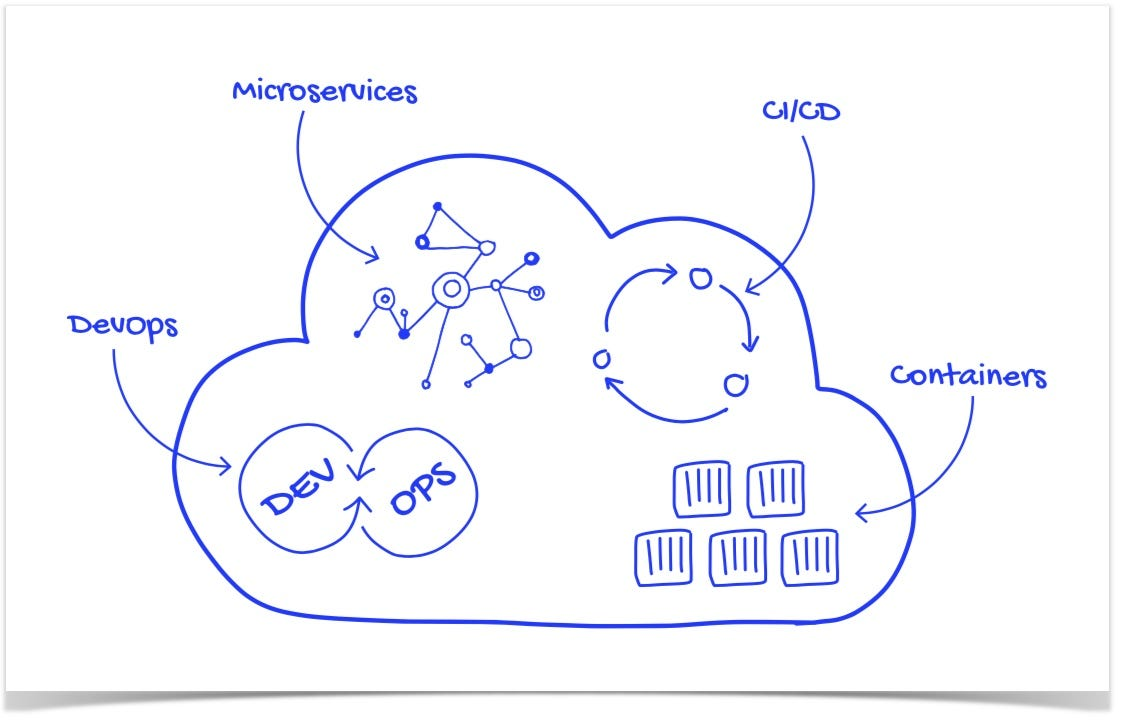
\includegraphics[width=0.6\textwidth]
    {Figures/cloud-native-architecture.jpg}
    \caption{Principal components of cloud-native architecture}
    \label{fig:cloud-native-architecture}
\end{figure}

DIS combines OCI infrastructure and managed services, including
networking, Object Storage, databases, and identity services, with custom
microservices deployed on Kubernetes. This architecture allows the
platform to support different analytics workloads while maintaining
scalability, tenant isolation, and operational reliability.

\subsection{Microservices Overview}
The DIS platform implements a comprehensive microservices-based architecture in which loosely coupled services communicate through RESTful APIs. All services are containerized and deployed on the Oracle Kubernetes Engine (OKE) platform, enabling scalability, fault tolerance, and independent service deployment.

Figure~\ref{fig:dis_microservices} illustrates the high-level microservices architecture of the DIS platform.

\begin{figure}[H]
    \centering
    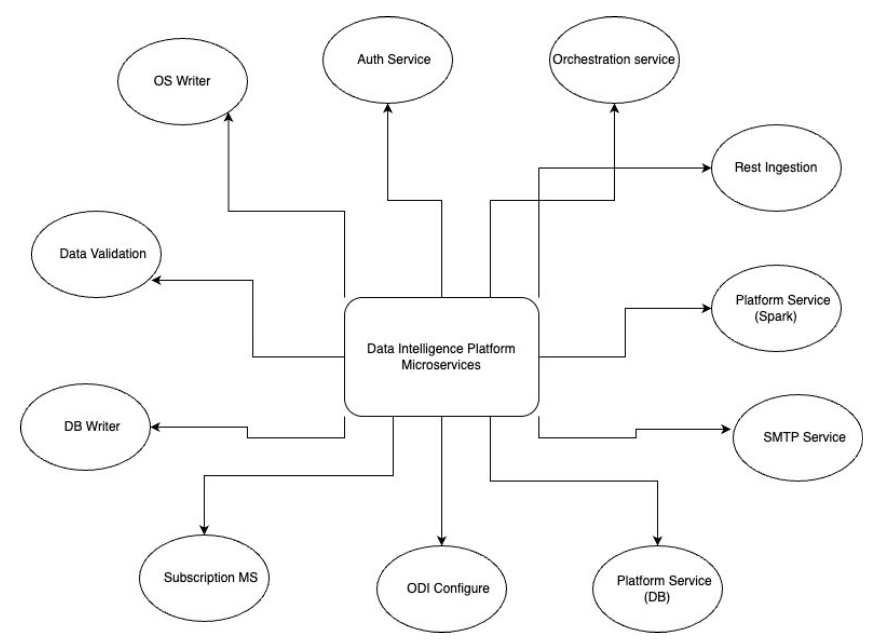
\includegraphics[width=0.8\textwidth]{Figures/dis_microservices.png}
    \caption{DIS Microservices Architecture}
    \label{fig:dis_microservices}
\end{figure}

\subsubsection{Orchestration Service}

The \textbf{Orchestration Service} is responsible for automating the entire lifecycle of platform components and tenant environments, including initial deployment, configuration, ongoing management, updates, and rollback operations. It coordinates these tasks using template-driven workflows and internal REST APIs, ensuring that all provisioning activities are executed consistently and reliably.

This microservice serves as the central coordinator of the DIS platform by orchestrating interactions among the different services involved in tenant onboarding and lifecycle management. By automating complex operational workflows, it minimizes manual intervention, improves deployment consistency, and enhances the overall reliability of the platform.

The features studied in this project involve the Orchestration Service together
with the configuration and OAC execution services. Their interaction is
examined in Chapter~\ref{chap:chapter3} through the cross-region disaster
recovery workflow.

\subsubsection{Authentication Service}

The \textbf{Authentication Service} is responsible for managing the secure onboarding and provisioning of tenant identities within the DIS platform. It enforces authentication, authorization, and compliance policies by integrating with Oracle Identity Cloud Service (IDCS) and partner platforms through standardized REST APIs.

This service plays a critical role in ensuring that only authenticated and authorized tenants can access DIS resources. Throughout the provisioning and tenant lifecycle management processes, the Orchestration Service interacts with the Authentication Service to validate partner credentials, provision tenant identities, and manage access permissions. This collaboration guarantees secure communication between services while maintaining compliance with the platform's security requirements.
\begin{figure}[H]
    \centering
    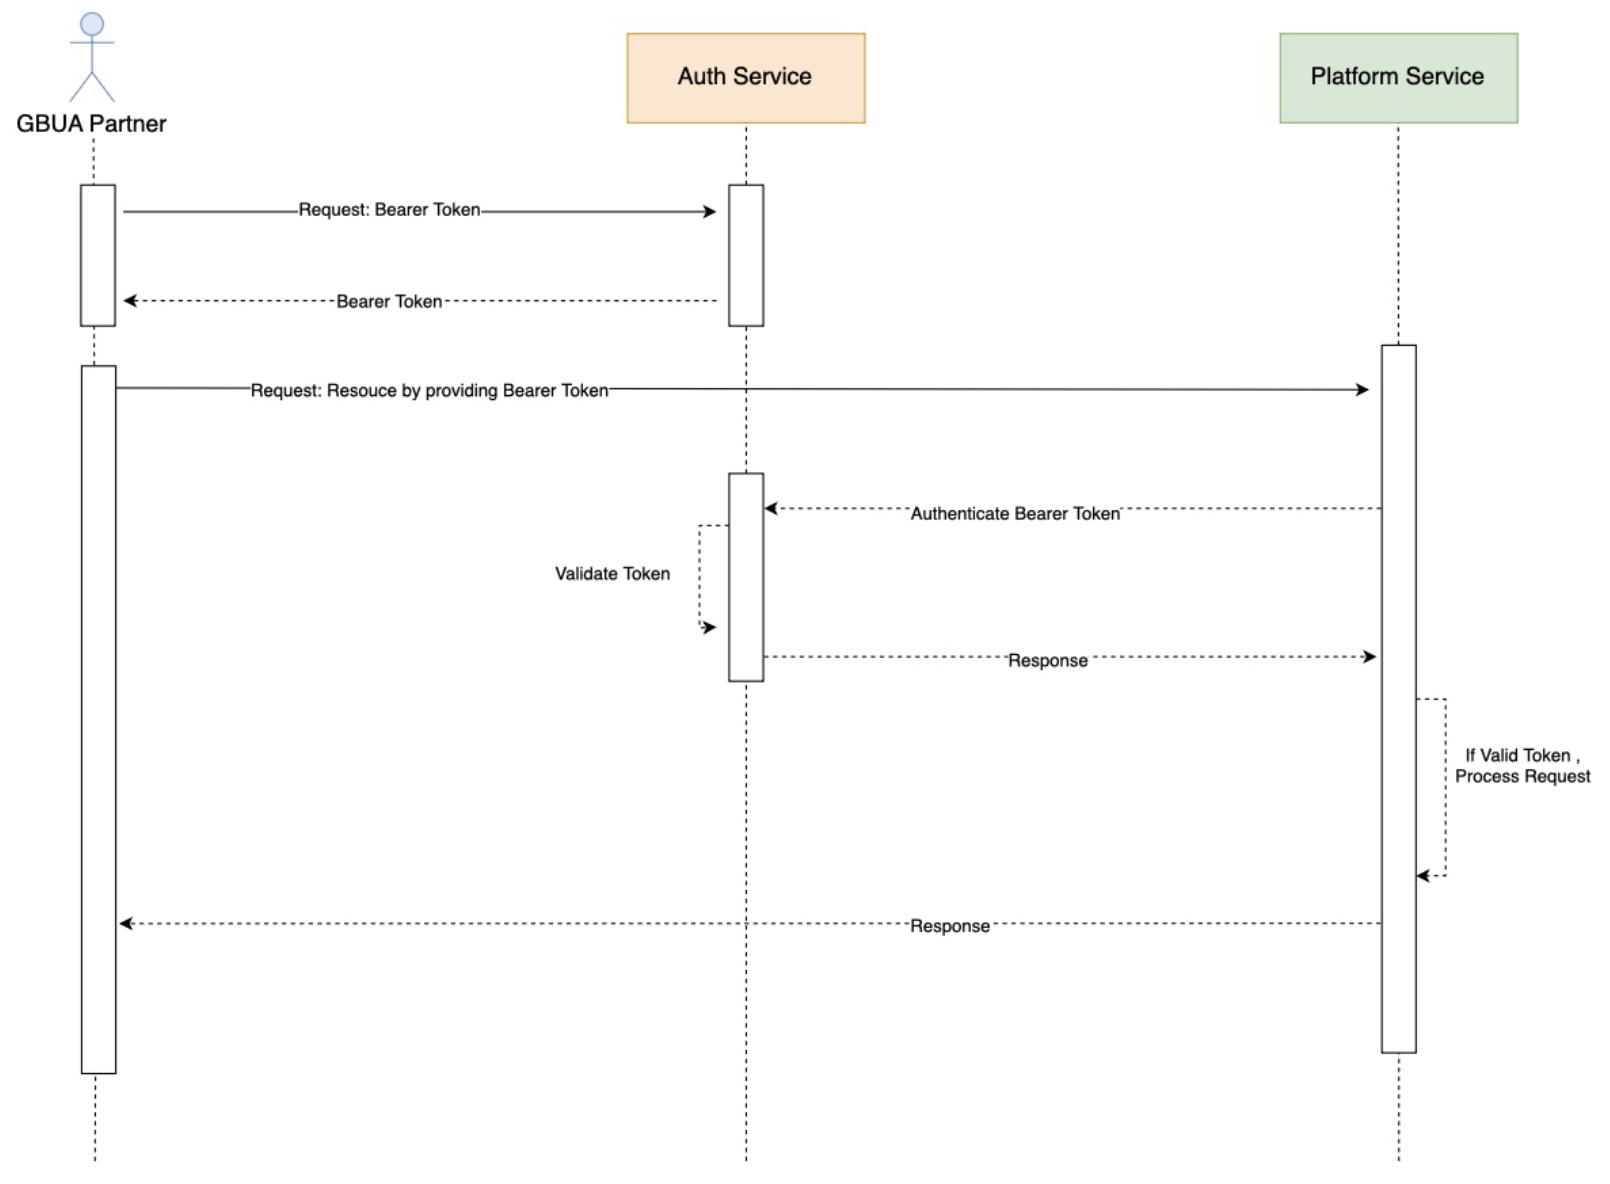
\includegraphics[width=0.8\textwidth]{Figures/Auth Service Sequence Diagram.png}
    \caption{Auth Service Sequence Diagram}
    \label{fig:Auth Service Sequence Diagram}
\end{figure}

\section*{Conclusion}

This chapter positioned DIS within Oracle and explained its role as a shared
analytics platform. It presented the partner and tenant operating model, the
provisioning lifecycle, the functional data flow, and the cloud-native
microservices architecture. These concepts establish the system context needed
to understand the technologies and OAC recovery solution presented in the next
chapter.
